\section{Metodología Experimental}
\subsection{Doble Rendija y Anillo de Airy}
Nuestro primer objetivo fue comparar las mediciones hechas en el laboratorio sobre las dimensiones de los patrones de difracción provocados por una doble rendija y por una perforación circular con las expresiones respectivas \eqref{eq: airy} y \eqref{eq: maxima}.

Para esto empleamos un láser rojo con una longitud de onda de \qty{633}{\nm}, apuntando sobre una rejilla de doble rendija con parámetros $a = \qtylist{.2; .3; .45}{\mm}$ y $b = \qty{.05}{\mm}$, y con apertura circular con diámetros $D = \qtylist{.2; .3;.4}{\mm}$. La luz transmitida fue después proyectada sobre una tapa de cartón a una distancia $r_0 = \qty{114\pm.05}{cm}$ de las rejillas. El arreglo experimental se muestra en la figura~\ref{fig: labo0}.
\begin{figure}[H]
	\centering
	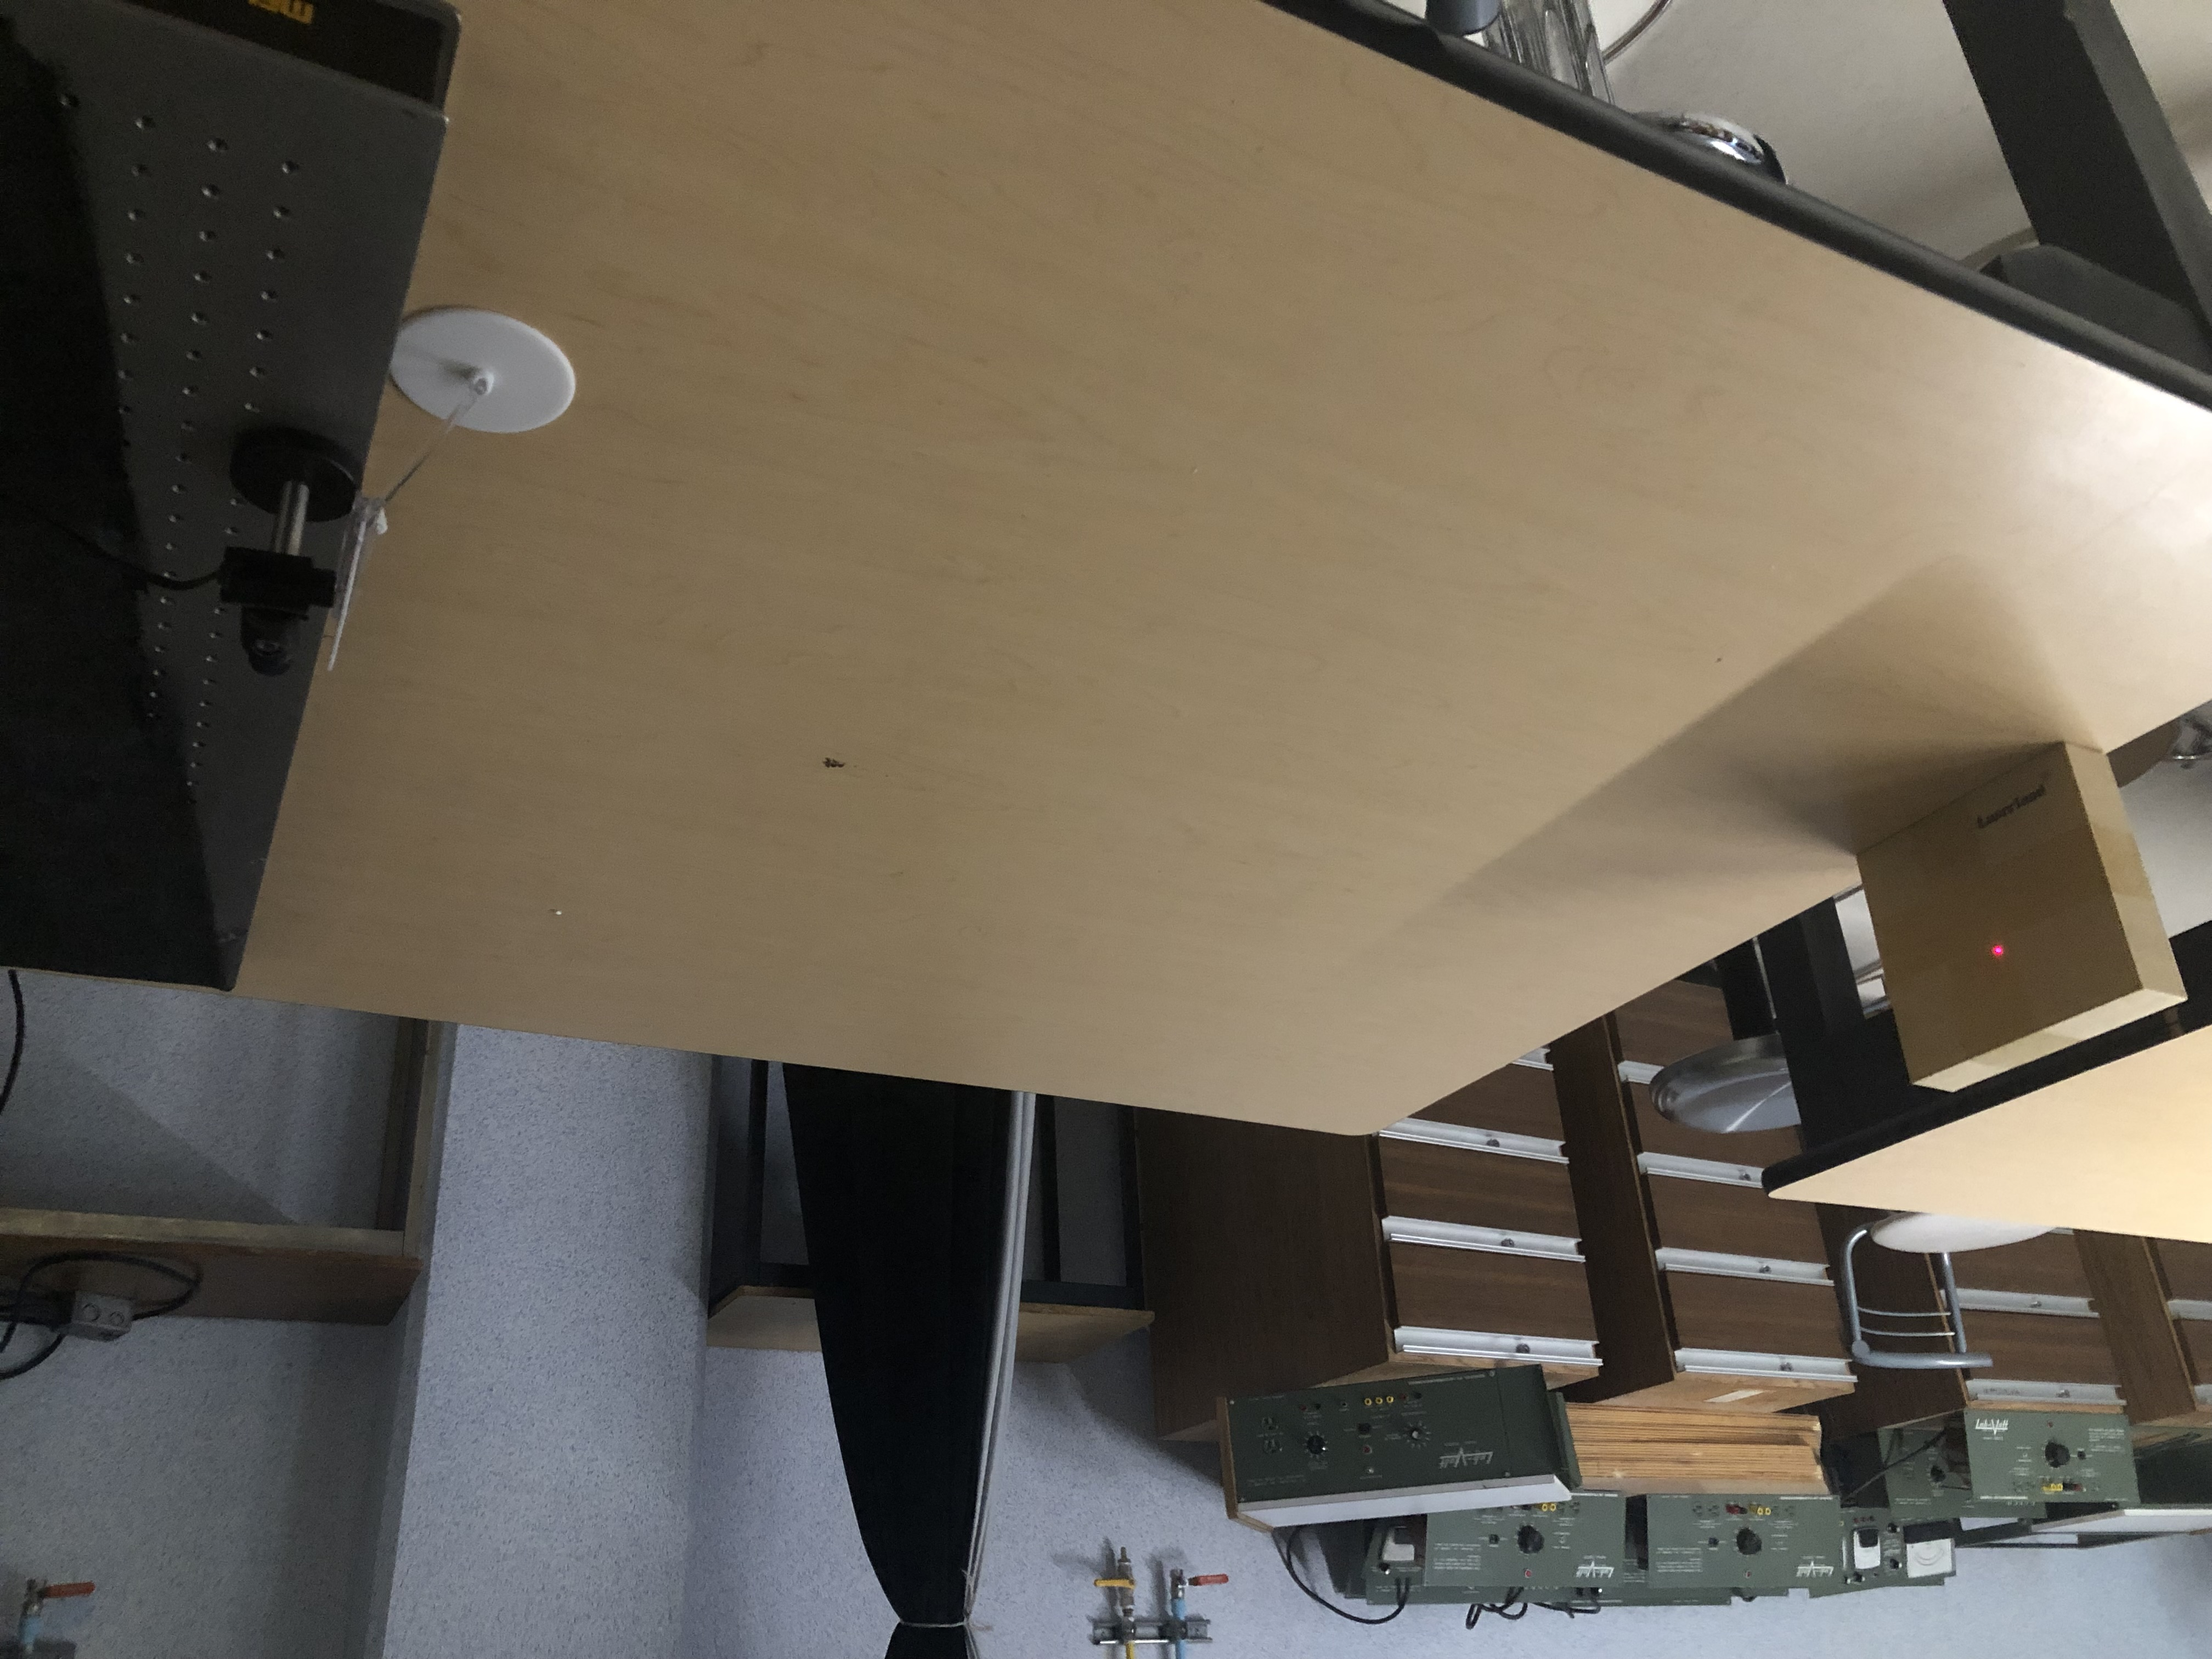
\includegraphics[width=.9\linewidth, angle=180]{Imagenes/labo0}
	\caption{Para tener una mejor apreciación entre las bandas brillantes al momento de medir sus separaciones se colocó la superficie de proyección a una distancia considerable y se disminuyó la intensidad de la iluminación en el laboratorio.}
	\label{fig: labo0}
\end{figure}

Las dimensiones relevantes se midieron con un vernier, asegurando así una presición de \qty{.001}{\cm} en las mediciones.

\subsection{Grosor del Cabello}\label{sec: hair}
Para medir el grosor de un cabello sustituimos la rejilla por un cabello tenso, sujetado a un marco con cinta masking, como se muestra en la figura~\ref{fig: hair}.
\begin{figure}[H]
	\centering
	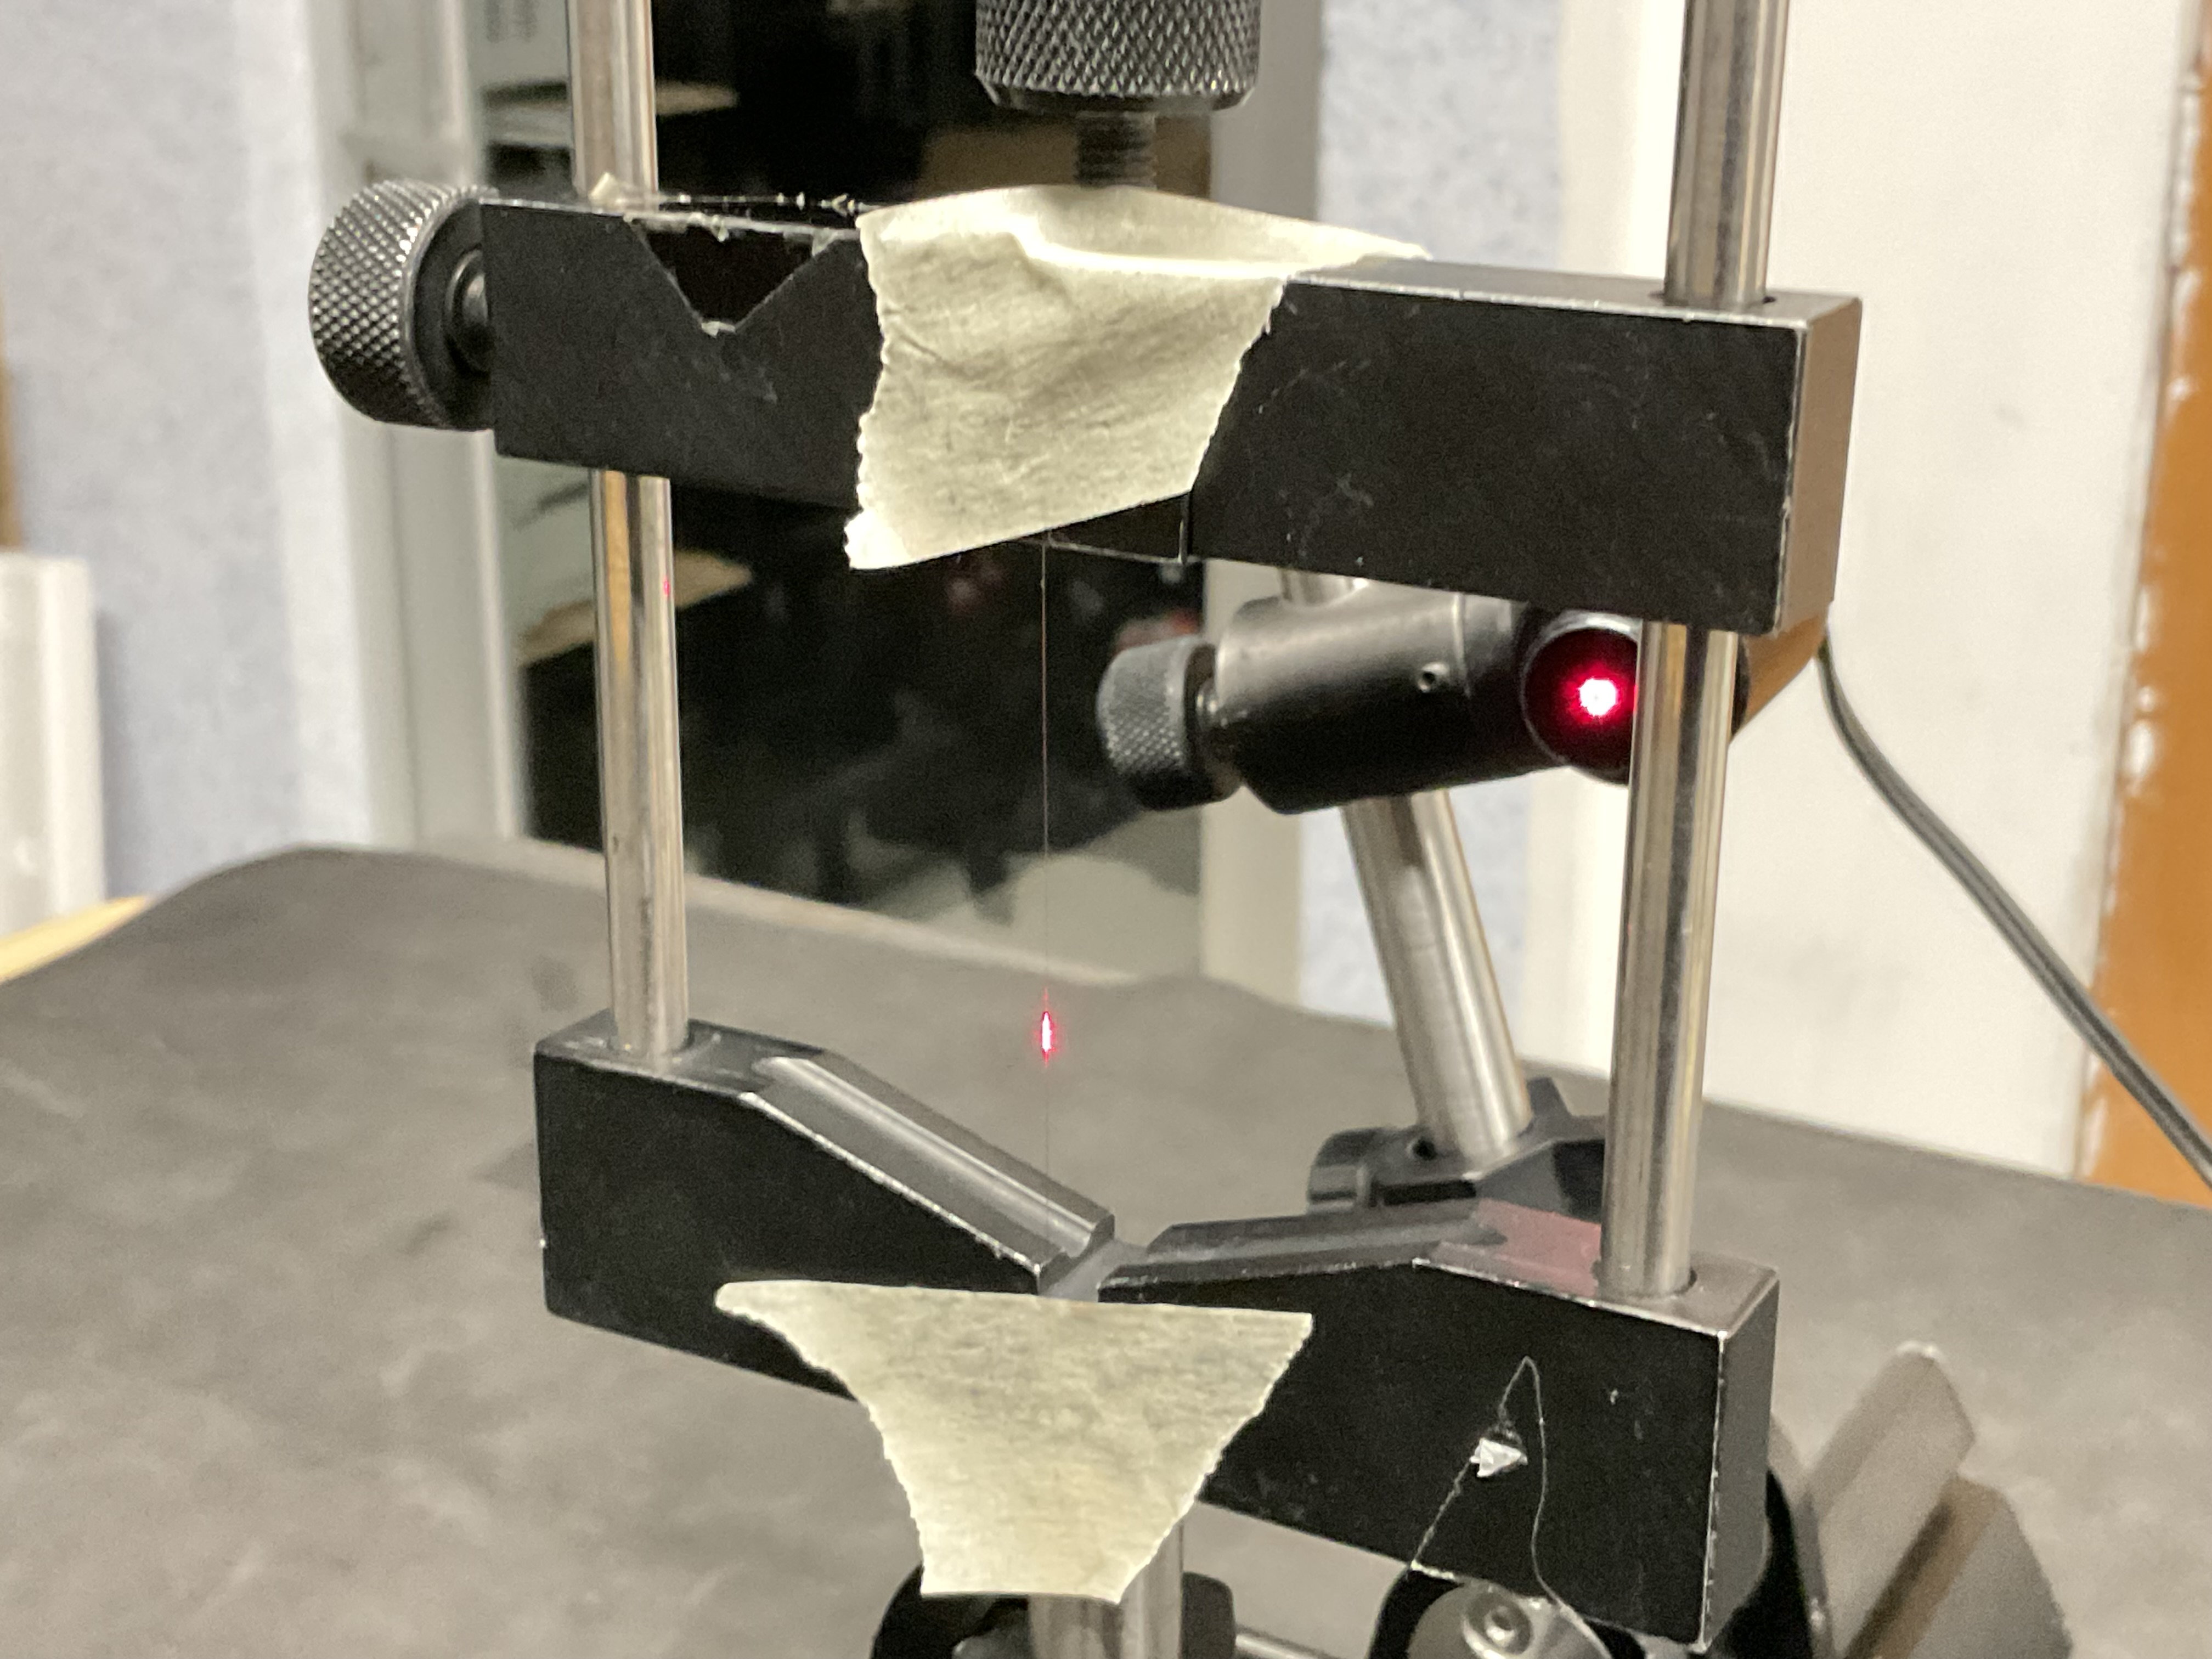
\includegraphics[width=.9\linewidth]{Imagenes/hair}
	\caption{}
	\label{fig: hair}
\end{figure}
En esta ocasión la pantalla de proyección fue una hoja de papel colocada a una distancia $r_0 = \qty{278.3}{\cm}$ del cabello.
\begin{figure}[H]
	\centering
	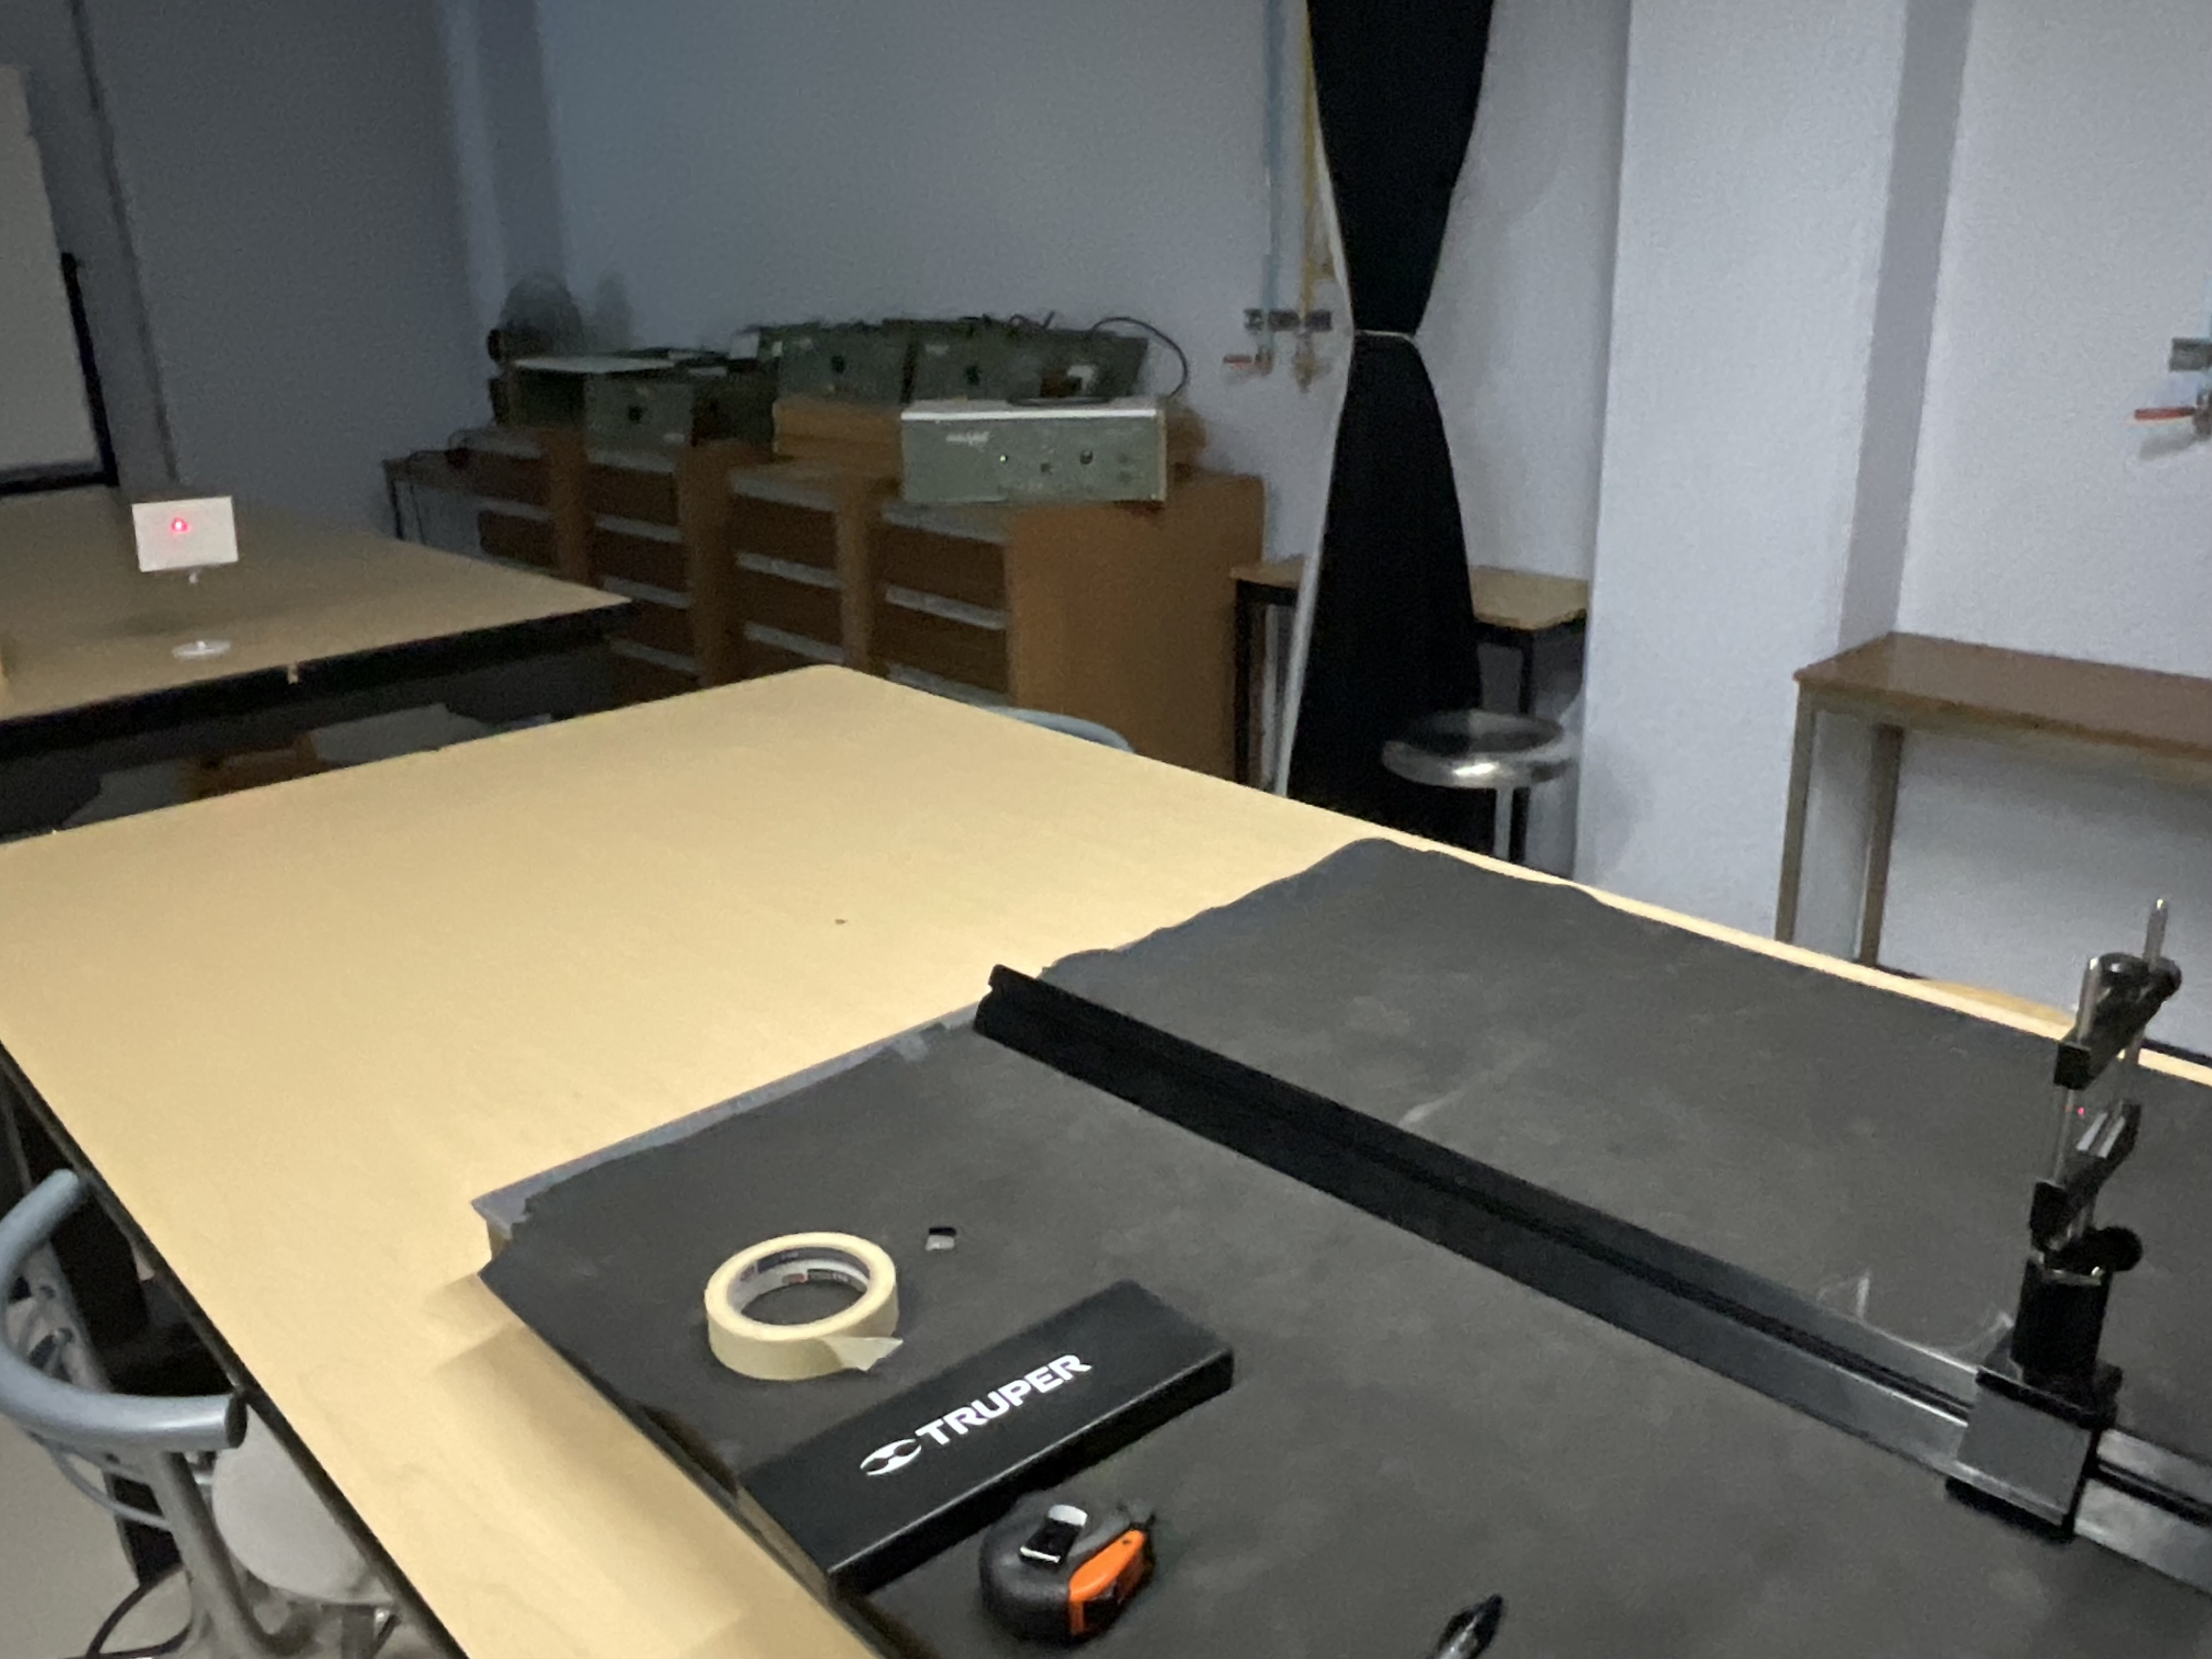
\includegraphics[width=.9\linewidth]{Imagenes/hair1}
	\caption{}
	\label{fig: hair1}
\end{figure}